% kuleuventheme2 by Janez Kren, September 2017, janez.kren@kuleuven.be, based on:
% kuleuventheme 1.3 by Roland Pastorino, 2013 roland.pastorino@kuleuven.be / www.rolandpastorino.com

\documentclass[11pt,t]{beamer}
\usetheme{kuleuven2}	%THEME OPTIONS for LOGO: kul (default), kulak, lrd,    ; OPTIONS for TITLE PAGE: normal (default), sedes


%%% OTHER SETTINGS
\usefonttheme[onlymath]{serif}			% math font with serifs, delete to make it sans-serif
\setbeamertemplate{footline}[body] 		% delete this line to remove footline bar on all frames
%\usepackage[orientation=landscape,size=custom,width=16,height=9,scale=0.5,debug]{beamerposter} %enable for widescreen 16:9 ratio



%%% ADDED PACKAGES:
\usepackage[english]{babel}
\usepackage{amsfonts}
\usepackage{amssymb}


%%% TITLE PAGE INFO:
\title[`AIMD' Simulations of Phosphate Hydrolysis Using NNPs]{\textit{Ab Initio} Molecular Dynamics Simulations of Phosphate Hydrolysis Using Neural Network Potentials} %[]] will appear in footline
\subtitle{Master's thesis defence presentation}
\setlength{\fboxrule}{0.3pt}
\setlength{\fboxsep}{0pt}
\titlegraphic{%
  \raisebox{-4.1cm}{\fbox{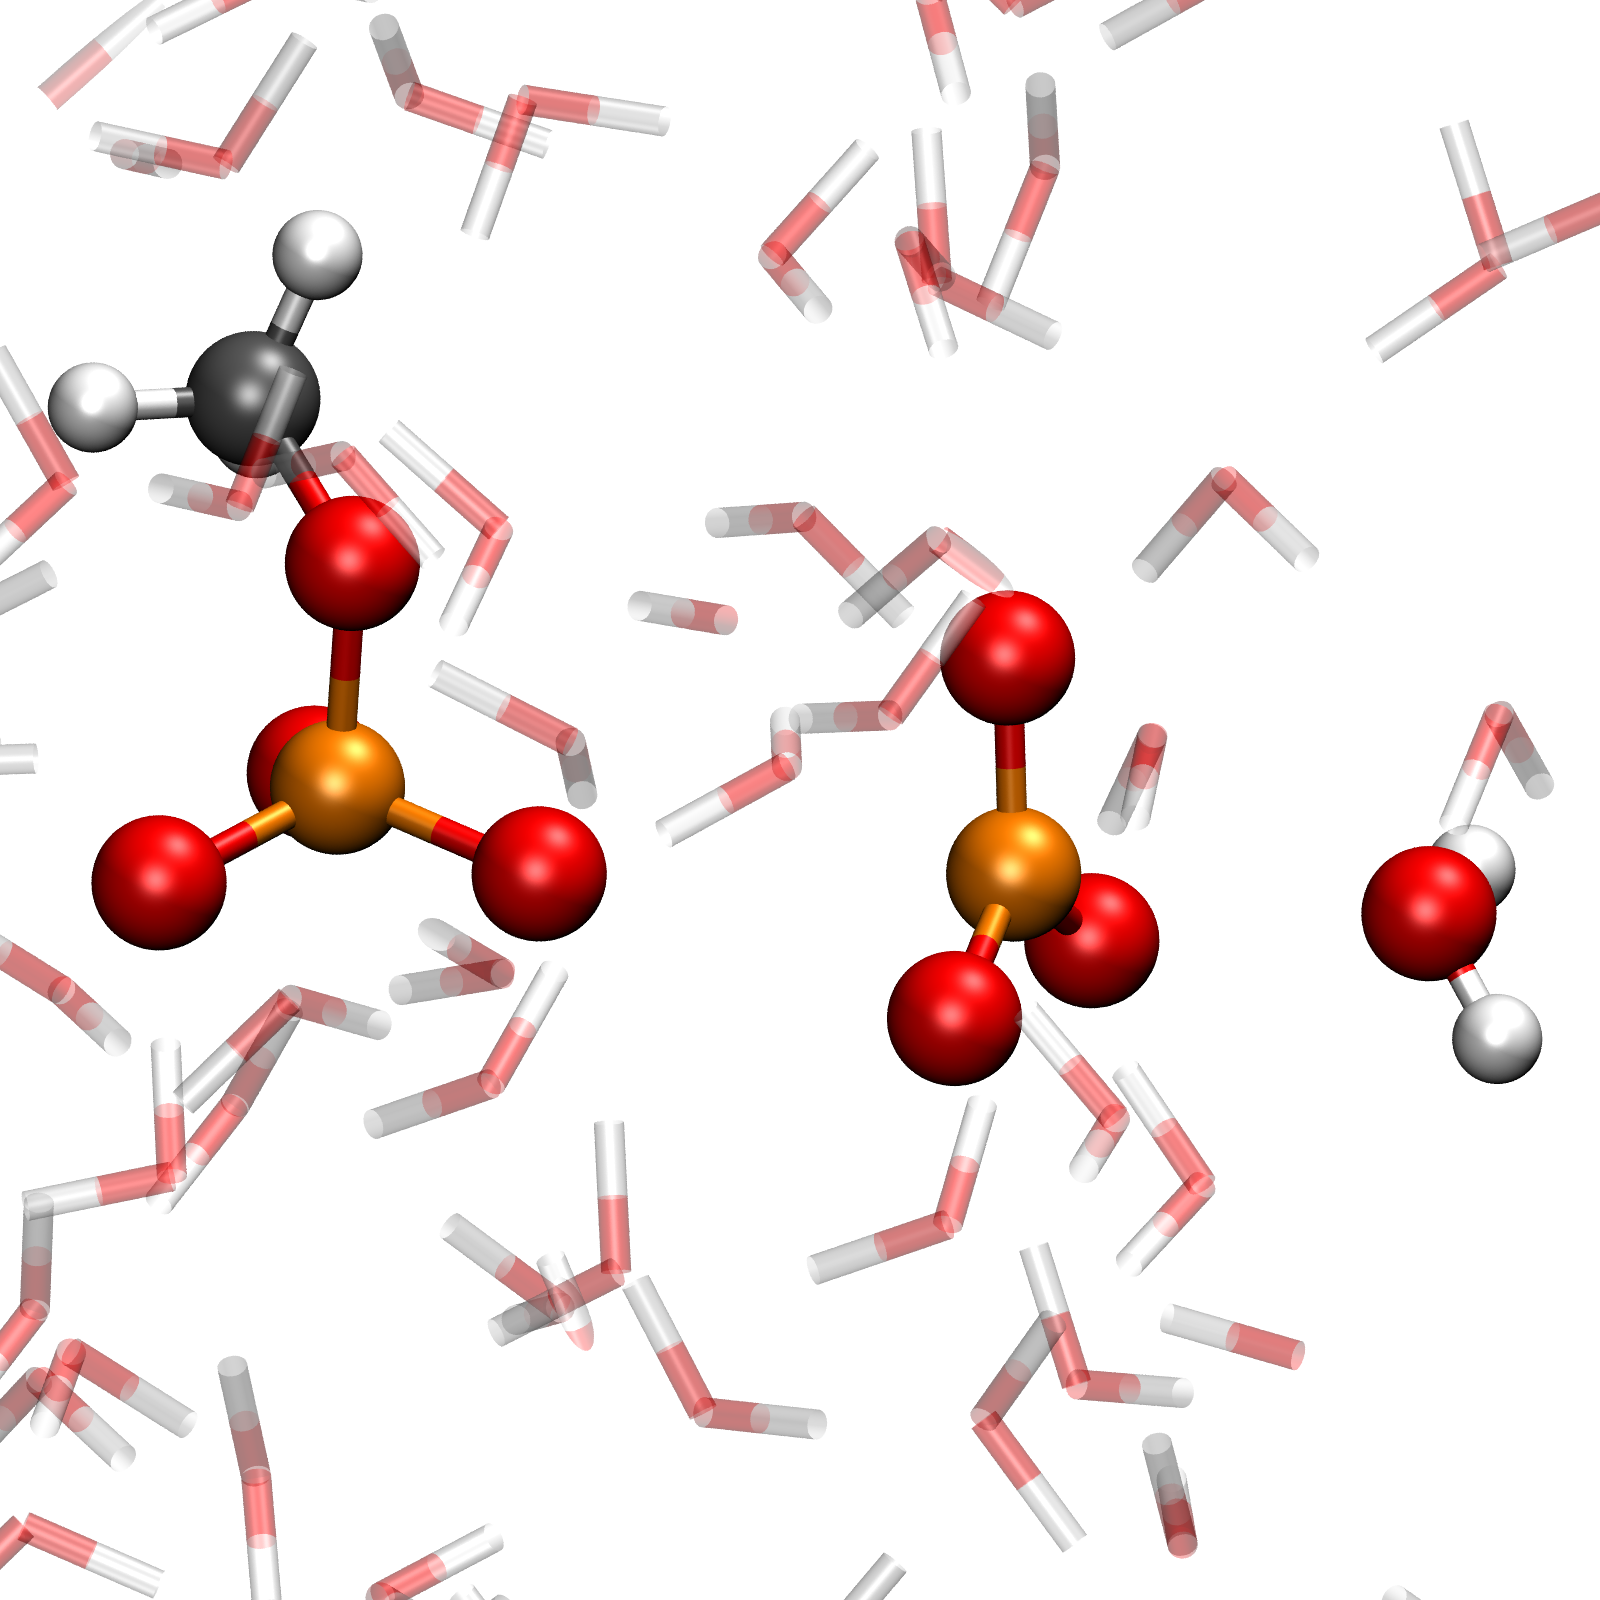
\includegraphics[width=.18\paperwidth]{Figures/MeDP_TSdissoc.png}}}
}
\author{Albert Makhmudov}
\institute{Supervisor: Prof. J. Harvey}
\date{June 2025}




\begin{document}
\csname beamer@calculateheadfoot\endcsname %recalculate head and foot dimension


 %%
 %%  0. TITLE PAGE and TABLE OF CONTENT
 %%
% Title page
\begin{frame}[plain,noframenumbering]
	\titlepage
\end{frame}



 %%
 %%  SECTION 1 - INTRODUCTION
 %%
\section{Introduction}
\begin{frame}{Why is phosphate hydrolysis challenging to study?}
	\vspace{-30pt}
	\begin{figure}
		\centering
		\includegraphics[width=0.9\textwidth]{Figures/introduction_background.png}
		\small
		\flushleft
		Would be nice to include a take-home message.
	\end{figure}
\end{frame}



\begin{frame}{Research goals}
	\small
	\begin{itemize}
		\item Compose a comprehensive dataset covering all reaction steps.
		\item Train the NequIP neural network to fit a neural network potential (NNP).
		\item Assess the accuracy and performance of the NNP.
		\item Perform well-tempered metadynamics simulations to obtain the free energy surface.
		\item Gain insights into the kinetics and thermodynamics of the reaction.
		\item Gain insights into the proton transfer mechanism.
	\end{itemize}	
\end{frame}



\begin{frame}
	\vspace{0.5cm}
	\begin{figure}
		\centering
		\includegraphics[width=0.23\textwidth]{Figures/introduction_paul_dirac.jpg}
	\end{figure}
	\small
	\begin{quotation}
		It therefore becomes desirable that approximate practical methods of applying quantum mechanics should be developed, which can lead to an explanation of the main features of complex atomic systems \textbf{without too much computation}.

		\raggedleft	\normalfont --  Paul Dirac
	\end{quotation}
\end{frame}



 %%
 %%  SECTION 2 - THEORETICAL BACKGROUND
 %%
\section{Theoretical background}
\begin{frame}{Geometric graph neural networks}
	\vspace{-10pt}
	\begin{figure}
		\centering
		\includegraphics[width=0.9\textwidth]{Figures/theory_geometric_gnns.png}
	\end{figure}
	\small
	Would be nice to include a take-home message.
\end{frame}



\begin{frame}{Neural equivariant interatomic potentials (NequIP)}
	\small
	The neural network is trained using a loss function:
	\begin{gather*}
		\mathcal{L} = \lambda_E \lVert \hat{E} - E \rVert^2 + \lambda_F \frac{1}{3N} \sum_{i=1}^{N} \sum_{\alpha=1}^{3} \left\lVert -\frac{\partial \hat{E}}{\partial r_{i,\alpha}} - F_{i,\alpha} \right\rVert^2
		\label{eq:loss_function}
	\end{gather*}
	It is based on a weighted sum of energy and force loss terms. Where $\hat{E}$ is the predicted energy, $\lambda_E$ and $\lambda_F$ are the energy and force weights, respectively, and $N$ is the number of atoms. MSE loss is used.
	\begin{figure}
		\centering
		\includegraphics[width=0.55\textwidth]{Figures/theory_nequip.png}
	\end{figure}
\end{frame}



\begin{frame}{Metadynamics}
	\vspace{-10pt}
	\begin{figure}
		\centering
		\includegraphics[width=0.9\textwidth]{Figures/theory_metadynamics.png}
	\end{figure}
	\small
	Would be nice to include a take-home message.
\end{frame}



 %%
 %%  SECTION 3 - METHODOLOGY
 %%
\section{Methodology}
\begin{frame}{System}
	\vspace{-5pt}
	\begin{figure}
		\centering
		\includegraphics[width=0.9\textwidth]{Figures/methods_collective_variables.png}
	\end{figure}
	\small
	The systems studied in this work are the following:
	\begin{itemize}
		\item MeDP$^{3-}$ with 3 Na$^+$ counterions solvated by 119 H$_2$O.
		\item MeHDP$^{2-}$ with 2 Na$^+$ counterions solvated by 124 H$_2$O.
	\end{itemize}
	The box dimensions are 15.877 $\times$ 15.877 $\times$ 15.877 and 15.901 $\times$ 15.901 $\times$ 15.901 \AA$^3$, respectively.
\end{frame}



\begin{frame}{Neural network training workflow}
	\vspace{-10pt}
	\begin{figure}
		\centering
		\includegraphics[width=1.0\textwidth]{Figures/methods_workflow_diagram.pdf}
	\end{figure}
\end{frame}



 %%
 %%  SECTION 3 - RESULTS
 %%
\section{Results}
\begin{frame}{Final training and test datasets' composition}
	\vspace{-10pt}
	\begin{figure}
		\centering
		\includegraphics[width=0.85\textwidth]{Figures/results_final_dataset_with_histograms.png}
	\end{figure}
	\small
	The final training and test datasets consist of 12,000 and 1,800 frames, respectively, and covers all reaction steps.
\end{frame}



\begin{frame}{Accuracy of the fitted potential}
	\begin{columns}[t]
		\begin{column}{.55\textwidth}
			\vspace{-20pt}
			\begin{figure}
				\centering
				\includegraphics[width=1.0\textwidth]{Figures/results_nnp_accuracy_l-1_l-2.png}
			\end{figure}	
		\end{column}
		\begin{column}{.45\textwidth}
			\small
			Community standards are as follows:
			\begin{itemize}
				\item `very good fit' \\
				\noindent $\text{MAE}_E = 1\text{-}10 \; \text{meV/atom}$ \\
				\noindent $\text{RMSE}_F = 20\text{-}40 \; \text{meV/\AA}$
				\item `perfect fit' \\
				\noindent $\text{MAE}_E \sim 1 \; \text{meV/atom}$ \\
				\noindent $\text{RMSE}_F \sim 10 \; \text{meV/\AA}$
			\end{itemize}
			We fitted 2 potentials and both of them are very accurate exhibiting fairly small errors.
		\end{column}
	\end{columns}	
\end{frame}



\begin{frame}{Performance of the potential}
	\vspace{-10pt}
	\begin{figure}
		\centering
		\includegraphics[width=0.6\textwidth]{Figures/results_performance_comparison.png}
	\end{figure}
	\small
	The turning point in choosing between the potentials with tensor ranks $\ell = 1$ and $\ell = 2$ is the performance. The $\ell = 1$ potential is about 2.5 times faster than the $\ell = 2$ potential, while the accuracy is comparable.
\end{frame}



\begin{frame}{Convergence of the free energy profiles}
	\begin{columns}[t]
		\begin{column}{.65\textwidth}
			\vspace{-25pt}
			\begin{figure}
				\centering
				\includegraphics[width=1.05\textwidth]{Figures/results_300K_fes_conv_cv_evol.png}
			\end{figure}	
		\end{column}
		\begin{column}{.35\textwidth}
			\vspace{-10pt}
			\small
			\begin{itemize}
				\item The profiles are not fully converged.
				\item Hence, the results should be considered provisional.
				\item There are recrossing events between the reactants and products states.
				\item Which gives confidence in the soon approaching convergence.
			\end{itemize}
		\end{column}
	\end{columns}
\end{frame}



\begin{frame}{Reaction mechanism for MeDP$^{3-}$ at 300 K}
	\vspace{-10pt}
	\begin{figure}
		\centering
		\includegraphics[width=0.9\textwidth]{Figures/results_MeDP_300K_fes_mfep.png}
	\end{figure}
	\small
	The more favourable reaction mechanism is a dissociative/concerted (D$_\text{N}$A$_\text{N}$) one. $\Delta G^\ddagger_\text{exp}$ for HP$_2$O$_7$$^{3-}$ hydrolysis at 25\textdegree{C} is 29.2 kcal/mol. The $\Delta G^\ddagger_\text{calc}$ of 28.22 kcal/mol is within the chemical accuracy!
\end{frame}



\begin{frame}
	\vspace{0.5cm}
	\begin{figure}
		\centering
		\includegraphics[width=1.0\textwidth]{Figures/results_MeDP_reaction_mechanism_steps.pdf}
	\end{figure}
\end{frame}

\begin{frame}[b]{Positioning}
Frame option [b] for text at the bottom of the frame
\vspace{8mm} %needed to aviod overlaying with footline
\end{frame}




\begin{frame}[plain,fragile]{Footline}   %option fragile needed for verbatim environment
\vspace{2.1mm} %extra space needed, otherwise text starts to close to the frame title
Frame option [plain] to remove footline on individual frame

\vspace{25pt}
To remove footline from \emph{all} frames delete this line from preamble in .tex file: 
	\begin{verbatim}
	\setbeamertemplate{footline}[body]
	\end{verbatim}
\end{frame}




\begin{frame}
	This frame has no title.
\end{frame}




\begin{frame}{Double--column frame}
	\begin{columns}[t]
		\begin{column}{.5\textwidth}
			This is the top of the first column.	
		\end{column}
		\begin{column}{.5\textwidth}
			This is the top of the second column.
		\end{column}
	\end{columns}	
\end{frame}




\begin{frame}{Text alignment}
	\begin{flushleft}
		Left justified 	environment ...
	\end{flushleft}
	\begin{center}
		Center environment ...
	\end{center}
	\begin{flushright}
		Right justified environment ...
	\end{flushright} 

\vspace{6pt}
\raggedright Ragged right command ...

\centering	Centering command ...

\raggedleft Ragged left command ...

\vspace{6pt}
\flushleft Flush left command ...

\flushright Flush right command ...
\end{frame}




\begin{frame}{Colour palette}
Recommended, predefined colours
\begin{itemize}
	\item black
	\item \textcolor{kul-blue}{KU Leuven primary blue}, \textcolor{kul-secblue}{secondary blue}, and \textcolor{kul-dark}{dark blue}
	\item \textcolor{white}{white} $\leftarrow$ white, when background is dark
	\item \textcolor{gray}{50\% gray }, for text and \textcolor{lgray}{5\% gray} for background

	\vspace{5mm}
	\item \textcolor{red}{red text colour}, used for \alert{alert text}
\end{itemize}
\end{frame} 




\begin{frame}{Font styles}
Sans-serif family of Modern Latin font
\begin{itemize}
	\item Normal text
	\item \textbf{Bold}
	\item \textit{Italic}, \emph{Emphasis}, \textsl{Slanted}
	\item \underline{Underline}
	\item \textsc{Small caps}
	\item \texttt{Typewriter}
\end{itemize}
\end{frame}




\begin{frame}{Font sizes}
\begin{itemize}
	\item \tiny tiny
	\item \scriptsize scriptsize
	\item \footnotesize footnotesize
	\item \small small
	\item \normalsize normalsize
	\item \large large
	\item \Large Large
	\item \LARGE LARGE
	\item \huge huge
	\item \Huge Huge 
\end{itemize}
\end{frame} 




\begin{frame}[fragile]{Equations and math}   %option fragile needed for verbatim environment
Equations and other mathematical symbols use serif typeface:
\begin{gather*}
f(x)= a x^2 + b x + c
\end{gather*}

Style of individual symbols can be changed manually:
\begin{gather*}
\mathbf{\hat{\beta}} = \underset{b}{\rm arg\,min}\,(\mathbf{y}- \mathbf{X} \mathbf{b})^{\mathsf{T}}\,\boldsymbol{\Omega}^{-1}(\mathbf{y}- \mathbf{X} \mathbf{b}) \\
\mathsf{    G_t = \alpha e^{-\beta e^{-\gamma \cdot t}}    }
\end{gather*}

To change all math into sans-serif delete this line from the preamble in .tex file:
	\begin{verbatim}
	\usefonttheme[onlymath]{serif}
	\end{verbatim}
\end{frame}




\begin{frame}{Graphics}
\vspace{-12pt}
	\begin{figure}
	\centering
	\includegraphics[width=0.6\textwidth]{example_figure.pdf}
	\caption{Example graphic \label{fig:figure1}}
	\footnotesize
	\flushleft
	Do not delete logo files in the graphics folder. They are used on the title page and in the footline.
	\end{figure}
\end{frame}




\begin{frame}{Tables}
\begin{table}
	\centering
	\scriptsize
	\caption{Example table}
	\begin{tabular}{lccc} \hline
	 & (1) & (2) & (3) \\ \hline
	$x_1$ & 0.705*** & 0.215** & 0.123 \\
	 & (0.107) & (0.0964) & (0.105) \\
	$x_2$ & 0.476*** &  & 0.114** \\
	 & (0.0489) &  & (0.0519) \\
	$x_3$ &  & 0.592*** & 0.538*** \\
	 &  & (0.0361) & (0.0436) \\
	Constant & 0.0478 & 0.0576 & 0.0511 \\
	 & (0.0487) & (0.0427) & (0.0426) \\
	 &  &  &  \\
	Observations & 500 & 500 & 500 \\
	 R-squared & 0.711 & 0.776 & 0.779 \\ \hline
	\end{tabular}
	
	\flushleft\scriptsize
	Standard errors in parentheses, *** p$<$0.01, ** p$<$0.05, * p$<$0.1
\end{table}
\end{frame}




\begin{frame}[fragile]{Widescreen}
	Default screen ration is 4:3.  Load the following package in the preamble to make all frames wider to 16:9 ratio:
	
	\begin{verbatim}
	\usepackage[orientation=landscape,size=custom,
	width=16,height=9,scale=0.5,debug]{beamerposter} 
	\end{verbatim}
	
	Title page or other frames should not get distorted because of it. 
	
	\begin{center}
		\begin{tikzpicture}[scale=0.2]
		\path [fill=lgray] (0,0) rectangle (12,9);
		\node [below, gray] at (6,0) {4:3};
		\draw [kul-blue, semithick] (0,0) rectangle (16,9);
		\node [above, kul-blue] at (8,9) {16:9};
		\end{tikzpicture}
	\end{center}
\end{frame}







 %%
 %%  SECTION 3 - ITEMIZATION
 %%
\section{Itemization and enumeration} \label{sec:items}
\begin{frame}{Itemize}
(default)
\begin{itemize}
	\item Itemize style
	\item Itemize style
	\begin{itemize}
		\item Itemize subitem
		\item Itemize subitem
			\begin{itemize}
				\item Itemize subsubitem
				\item Itemize subsubitem
			\end{itemize}
		\item Itemize subitem	
	\end{itemize}
	\item Itemize style
\end{itemize}
\end{frame}




\begin{frame}{Itemize}
(extra space between items)
\begin{itemize}
	\itemsep 20pt
	\item Itemize style
	\item Itemize style
	\begin{itemize}
		\itemsep 10pt
		\item Itemize subitem
		\item Itemize subitem
		\item Itemize subitem	
	\end{itemize}
	\item Itemize style
\end{itemize}
\end{frame}




\begin{frame}{Enumerate}
(default)
\begin{enumerate}
	\item Enumerate style
	\item Enumerate style
	\begin{enumerate}
		\item Enumerate subitem
		\item Enumerate subitem
		\begin{enumerate}
			\item Enumerate subsubitem
			\item Enumerate subsubitem
		\end{enumerate}
		\item Enumerate subitem
	\end{enumerate}
	\item Enumerate style
\end{enumerate}
\end{frame}




\begin{frame}{Enumerate}
(option I) + pause
\begin{enumerate}[I]
	\item Enumerate style
	\item Enumerate style
	\begin{enumerate}[I]
		\item Enumerate subitem
		\item Enumerate subitem
		\pause
		\begin{enumerate}[I]
			\item Enumerate subsubitem
			\item Enumerate subsubitem
		\end{enumerate}
		\pause
		\item Enumerate subitem
	\end{enumerate}
	\item Enumerate style
\end{enumerate}
\end{frame}




\begin{frame}{Enumerate}
(option i.)
\begin{enumerate}[i.]
	\item Enumerate style
	\item Enumerate style
	\begin{enumerate}[i.]
		\item Enumerate subitem
		\item Enumerate subitem
		\begin{enumerate}[i.]
			\item Enumerate subsubitem
			\item Enumerate subsubitem
		\end{enumerate}
		\item Enumerate subitem
	\end{enumerate}
	\item Enumerate style
\end{enumerate}
\end{frame}




\begin{frame}{Enumerate}
(option A.) + effects
\begin{enumerate}[A.]
	\item<1-5> Enumerate style
	\item<1-5> Enumerate style
	\begin{enumerate}[A.]
		\item<2-5> Enumerate subitem
		\item<3-5> Enumerate subitem
		\begin{enumerate}[A.]
			\item<3-4> Enumerate subsubitem
			\item<3-4> Enumerate subsubitem
		\end{enumerate}
		\item<4-5> Enumerate subitem
	\end{enumerate}
	\item<5> Enumerate style
\end{enumerate}
\end{frame}




\begin{frame}{Enumerate}
(option a + extra space)
\begin{enumerate}[a\enspace]
	\item Enumerate style
	\item Enumerate style
	\begin{enumerate}[a\enspace]
		\item Enumerate subitem
		\item Enumerate subitem
		\begin{enumerate}[a\enspace]
			\item Enumerate subsubitem
			\item Enumerate subsubitem
		\end{enumerate}
		\item Enumerate subitem
	\end{enumerate}
	\item Enumerate style
\end{enumerate}
\end{frame}








 %%
 %%  SECTION 4 - OTHER
 %%
\section{Blocks and other environments}	\label{sec:blocks}
\begin{frame}{Theorems and other blocks}
	\begin{block}{Title of the bloc}
	Text for generic block
	\end{block}

\vspace{11pt}
	\begin{exampleblock}{Example block title}
	Text for example block
	\end{exampleblock}

\vspace{11pt}
	\begin{alertblock}{Alert block title}
	Text for alert block
	\end{alertblock}
\end{frame}




\begin{frame}{Theorems and other blocks}
Theorem environment
	\begin{theorem}
		$a^2 + b^2 = c^2$
	\end{theorem}

\vspace{11pt}
Definition environment
	\begin{definition}
		Here is definition text
	\end{definition}

\vspace{11pt}	
Example environment
	\begin{example}
		Example text
	\end{example}
\end{frame}




\begin{frame}{Theorems and other blocks}
Proof environment
	\begin{proof}
	Proof text.
	\end{proof}
	
	\begin{proof}[Proof with custom title\nopunct]
	Proof with any name and optionally without full stop in the title
	\end{proof}

\vspace{11pt}	
Corollary environment
	\begin{corollary}
	$ x + y = y + x  $
	\end{corollary}
\end{frame}




\begin{frame}{Boxes}
'Beamer color box' with five different pre-set colour combinations
	\begin{center}~
	% box1 = kul-blue background and white text
		\begin{beamercolorbox}[wd=.7\textwidth,sep=4pt,center]{box1}
		box1 scheme
		\end{beamercolorbox}
	\end{center}
	
	\begin{center}~
	% box2 = light gray background and kul-blue text
		\begin{beamercolorbox}[wd=.7\textwidth,sep=4pt,center]{box2}	
		box2 scheme  \\
				second line
		\end{beamercolorbox}
	\end{center}
	
	\begin{center}~
	% box3 = light gray background and black text
		\begin{beamercolorbox}[wd=0.3\textwidth,sep=4pt,right]{box3}
		box3 scheme, aligned right
		\end{beamercolorbox}
	\hspace{11pt}
	% box4 = light gray background and red text
		\begin{beamercolorbox}[wd=0.3\textwidth,sep=4pt]{box4}		
		box4 scheme, aligned left
		\end{beamercolorbox}
	\end{center}
	
	\begin{center}~
	% box5 = red background and white text
		\begin{beamercolorbox}[wd=2cm,ht=1.5cm,sep=4pt,center]{box5}
		box5
		\\
		 \
		\end{beamercolorbox}
	\end{center}

\end{frame}




\begin{frame}{Quotes}
Quote 
\begin{quote}
	Quote environment is for a short quotation, or a series of small quotes, separated by blank lines.
\end{quote}

\vspace{11pt}
Quotation 
\begin{quotation}
	Quotation environment is for use with longer quotations, of more than one paragraph, because it indents the first line of each paragraph. 

	Quotation environment is for use with longer quotations, of more than one paragraph, because it indents the first line of each paragraph.
	
	\raggedleft	\normalfont --  WikiBooks \LaTeX$ $ guide
\end{quotation}
\end{frame}




\begin{frame}[fragile]{Quotes}
Verse
\begin{verse}
	Verse environment \\ 
	is for quotations where \\
	line breaks are important. 
\end{verse}

\vspace{11pt}
Verbatim
\begin{verbatim}
Verbatim text is ideal for typesetting program
source code. To use it in Beamer the frame needs
option [fragile].
\end{verbatim}
\end{frame}




\begin{frame}
\vspace{15pt}
Abstract environment
\begin{abstract}
	Lorem ipsum dolor sit amet, consectetur adipiscing elit. Pellentesque quis pharetra sapien, non tempor tortor. Vestibulum gravida mauris ac lorem semper, vel vulputate mauris tincidunt. Sed diam ante, dignissim consequat pulvinar in, placerat eu nibh. Donec congue id elit sit amet iaculis.
	
	Proin pellentesque vel ex in fermentum. Pellentesque suscipit odio ut accumsan feugiat. Aliquam erat volutpat. Sed feugiat cursus eros, sit amet vestibulum ipsum pulvinar at. Sed eget porttitor purus. Duis nec nunc ex. Vestibulum ante ipsum primis in faucibus orci luctus et ultrices posuere cubilia Curae.
\end{abstract}
\end{frame}




\begin{frame}[label=buttons]{Buttons}
Standard buttons

	\hyperlink{fig:figure1}{\beamerbutton{Link to Figure 1}}

	\hyperlink{extraframe}{\beamergotobutton{Extra frame}}

	\beamerskipbutton{Button with long title and no link}

	\beamerreturnbutton{}

\vspace{11pt}
These buttons can link to any frame, figure, table, theorem, section, or anything else with defined label
\end{frame}




\begin{frame}[c,plain,noframenumbering]
\begin{tikzpicture}[remember picture,overlay]
\fill[fill=kul-blue]
    (current page.south east)  rectangle  ([shift={(0,-0.1\paperheight)}]current page.north west)   ;
\end{tikzpicture}

\centering
\textcolor{white}{Ending frame (version 1)}
\end{frame}




\begin{frame}[c,plain,noframenumbering]
\begin{tikzpicture}[remember picture,overlay]
\fill[fill=black]
    (current page.south east)  rectangle  (current page.north west)   ;
\end{tikzpicture}

\centering
\textcolor{white}{Ending frame (version 2)}
\end{frame}



\appendix
\begin{frame}[noframenumbering,label=extraframe]{Extra slide}
Because of frame option [noframenumbering] this frame is not counted in the total number of frames.

\vspace{24pt}
This button with cross-referencing link that will take you back to the frame: 

\hyperlink{buttons}{\beamerreturnbutton{Back to Buttons}}
\end{frame}


\end{document}